% Block diagram of the cache controller. Build: make diagrams  (-> diagrams/block_diagram.svg/.png, report/figures/block_diagram.pdf)
\documentclass[tikz,border=6pt]{standalone}
\usepackage{lmodern}\renewcommand{\ttdefault}{cmtt}
\usetikzlibrary{positioning,arrows.meta,calc,fit}
\DeclareRobustCommand{\code}[1]{\texttt{\detokenize{#1}}}
\tikzset{
  blk/.style={draw,rounded corners=2pt,align=center,minimum height=0.85cm,minimum width=2.1cm,fill=gray!8,font=\scriptsize},
  st/.style={draw,circle,align=center,minimum size=1.35cm,inner sep=1pt,fill=gray!8,font=\scriptsize},
  ar/.style={-{Stealth[length=2mm]},thick},
  lb/.style={font=\tiny,inner sep=1pt,fill=white}
}
\begin{document}
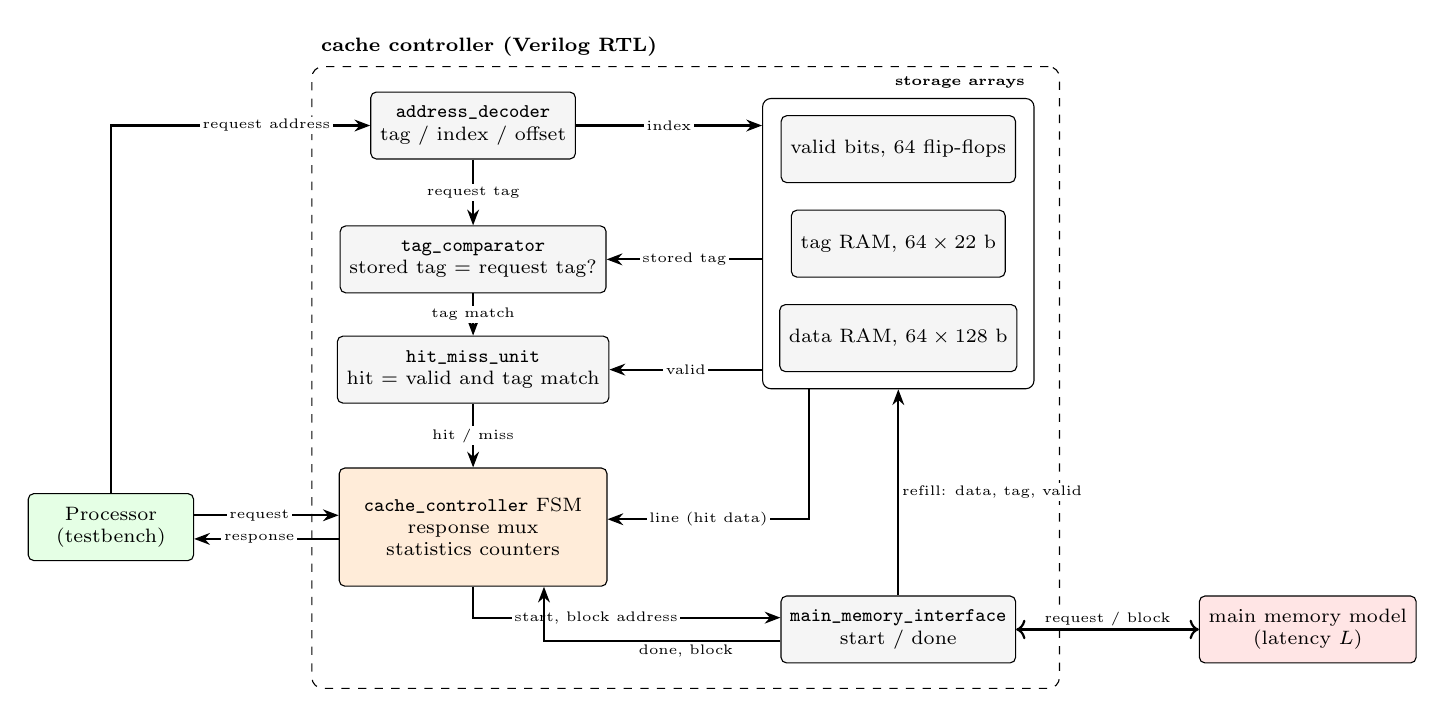
\begin{tikzpicture}[x=1cm,y=1cm]
  \node[blk,fill=green!10] (cpu) at (0,-1.9) {Processor\\(testbench)};
  \node[blk] (dec) at (4.6,3.2) {\code{address_decoder}\\tag / index / offset};
  \node[blk] (cmp) at (4.6,1.5) {\code{tag_comparator}\\stored tag = request tag?};
  \node[blk] (hm)  at (4.6,0.1) {\code{hit_miss_unit}\\hit = valid and tag match};
  \node[blk,fill=orange!15,minimum width=3.4cm,minimum height=1.5cm] (fsm) at (4.6,-1.9) {\code{cache_controller} FSM\\response mux\\statistics counters};
  \node[blk] (val) at (10,2.9) {valid bits, 64 flip-flops};
  \node[blk] (tag) at (10,1.7) {tag RAM, $64\times22$ b};
  \node[blk] (dat) at (10,0.5) {data RAM, $64\times128$ b};
  \node[draw,rounded corners=3pt,fit=(val)(tag)(dat),inner sep=6pt] (arr) {};
  \node[font=\tiny\bfseries,anchor=south east] at (arr.north east) {storage arrays};
  \node[blk] (mif) at (10,-3.2) {\code{main_memory_interface}\\start / done};
  \node[blk,fill=red!10] (mem) at (15.2,-3.2) {main memory model\\(latency $L$)};
  \node[draw,dashed,rounded corners=4pt,fit=(dec)(cmp)(hm)(fsm)(arr)(mif),inner sep=9pt] (box) {};
  \node[font=\scriptsize\bfseries,anchor=south west] at (box.north west) {cache controller (Verilog RTL)};
  \draw[ar] (cpu.north) |- node[lb,pos=0.8]{request address} (dec.west);
  \draw[ar] ([yshift=0.15cm]cpu.east) -- node[lb,pos=0.45]{request} ([yshift=0.15cm]fsm.west);
  \draw[ar] ([yshift=-0.15cm]fsm.west) -- node[lb,pos=0.55]{response} ([yshift=-0.15cm]cpu.east);
  \draw[ar] (dec.east) -- node[lb,pos=0.5]{index} (arr.west |- dec.east);
  \draw[ar] (dec.south) -- node[lb,pos=0.5]{request tag} (cmp.north);
  \draw[ar] (arr.west |- cmp.east) -- node[lb,pos=0.5]{stored tag} (cmp.east);
  \draw[ar] (arr.west |- hm.east) -- node[lb,pos=0.5]{valid} (hm.east);
  \draw[ar] (cmp.south) -- node[lb,pos=0.5]{tag match} (hm.north);
  \draw[ar] (hm.south) -- node[lb,pos=0.5]{hit / miss} (fsm.north);
  \draw[ar] ([xshift=0.6cm]arr.south west) |- node[lb,pos=0.75]{line (hit data)} ([yshift=0.1cm]fsm.east);
  \draw[ar] (fsm.south) |- node[lb,pos=0.7]{start, block address} ([yshift=0.15cm]mif.west);
  \draw[ar] ([yshift=-0.15cm]mif.west) -| node[lb,pos=0.2,below]{done, block} ([xshift=0.9cm]fsm.south);
  \draw[ar] (mif.north) -- node[lb,right]{refill: data, tag, valid} (arr.south);
  \draw[ar,<->] (mif.east) -- node[lb,pos=0.5,above]{request / block} (mem.west);
\end{tikzpicture}
\end{document}
